
%%\begin{abstract}
		%Pat's original email
		%In our experiment (CLAS12 at Jefferson Lab), we have event generators that simulate a large number of particle physics events, each of which consist of a number of kinematic variables.
		%The output of these event generators are then passed to another simulation framework that simulates these generated events in the detector geometry of the experiment. 
		%This latter process is very time-consuming given the large number of events that we want to reconstruct in our detectors.
		%We would like to develop a machine learning project that can train on the generated events and reconstructed events, and then predict the output of reconstruction based on the kinematic variables of the generated event.
		%This would allow us to reconstruct only a small amount of generated events through the reconstruction framework, thus drastically reducing the computing time needed for our research.
%% 		An electron-proton scattering experiment has been performed in the CLAS12 detector at the Thomas Jefferson National Accelerator Facility in order to probe the three-dimensional structure of the proton.
%%         Yields of scattered particles into the detector are determined by the types of interactions between incoming electrons and stationary protons.
%%         To understand the underlying physical processes observed in the experiment, the detector acceptance, which is the ratio of the number of events that are detected to the number that are produced, should be precisely estimated. 
%% 		The traditional method is to generate simulated data describing physical processes based on existing knowledge, then to pass these events to the Geant4 software package to simulate their interactions in the detector material.
%% 		A novel method to predict the output of reconstruction based on the kinematic variables of the generated events is described in this project.
%% 		This work is expected to drastically reduce the computing time needed for detector acceptance studies.
%%\end{abstract}


% Evaluation metrics for project proposal (10 points)
% Previous work and references: 2 points
% Understanding the problem, it’s formulation, and goal: 2 points
% Dataset to be used or collected, method or algorithm proposed: 2 points
% Well defined evaluation criteria: 2 points
% Writing clarity and structure: 2 points

% Questions you may answer when writing your proposal:
% What do you want to do? What question are you answering?
% What data will you use? Give a specific description of the data
% and confirm that you already have the data in hand at this point.
% What is your motivation? Formulate your problem as a machine learning problem.
% What methods will you try and compare?
% What computational resources will you use? Think about time and feasibility.
% Relevant related work? (brief summary)
% What is your project plan? You may include key steps and rough internal deadlines for each step.
% What are the risks? What might turn out to be more difficult than you anticipated? And how might you mitigate these risks?
%\linenumbers

%\section{Proposal}
% What do you want to do? What question are you answering?
Large scale particle physics experiments use humankind's largest machines to study nature at the smallest scales. One such experiment, called CLAS12 in Virginia at the Thomas Jefferson National Accelerator Facility (JLab) (\citet{BURKERT2020163419}), collides ultrarelativistic electrons moving only 1 m/s slower than the speed of light into an ultracold bunch of hydrogen to glean information about the substructure of the proton. The electrons interact with protons as described by quantum field theory, which can produce photons that, along with the starting electron and proton, are known as a final state. In particular, two photons, one electron and one proton in the final state is known as Deeply Virtual $\pi^0$ Production (DV$\pi^0$P), and this process is currently under detailed study as its properties are related to the mechanical properties of the proton (\citet{PhysRevD.55.7114}). 

%This is a continuation of the above paragraph, getting to answering "what is it you want to do" - I think what we need to answer is - we want to repalce GEANT4 with a generative model" 
The purpose of the CLAS12 detector is to detect the individual particles of this and other final states by recording the electrical signals produced when they pass through specific materials, which are then stored digitally and analyzed with reconstruction algorithms. In practice, there are many difficulties in reliably detecting and reconstructing particle paths, so computational methods have been developed to better understand detector and analysis algorithm's responses. Typically, real data is compared with the output of detailed simulations of the experiment, wherein Monte-Carlo (MC) methods are used to walk simulated particles through a detector system in many small time steps (\citet{PhysRevLett.115.212003, 10.1093/ptep/ptaa104}). However, this simulation method is very computationally expensive, especially for our particular physics experiment and process. Our goal is to use a generative machine learning model to mimic the output of the MC simulation and reconstructions, thus reducing computation time.


% What data will you use? Give a specific description of the data
% and confirm that you already have the data in hand at this point.
The standard simulation consists of two steps. First, we generate a data set of particle features - momenta and other properties - based on a combination of field-theoretic functions and empirical physics models, which creates an 'event' of a realistic four-particle final state from the DV$\pi^0$P process. This generation is very simple once the physics process has been defined, and well known and studied generators already exist\footnote{https://github.com/JeffersonLab/clas12-mcgen/}, and are very computationally inexpensive - 1 million events can be produced in less than a minute. The second step is for each event, walk all four particles through the simulated detector setup using the GEANT4 package (\citet{AGOSTINELLI2003250}). The output from this step is our four particles that we began with, but with their features smeared out. This second step is the one we are trying to supplement, as it would take about 5,000 hours on a single core machine to process 1 million events. However, through HPCC we have produced so far 100 M generated (step 1) and simulated (step 2) events that can be used for algorithmic training. 


% What is your motivation? Formulate your problem as a machine learning problem.
To describe the data structure, we start from a toy model, a baseball game with one pitcher and one catcher. In one ``inning", the pitcher throws a ball four times in a row, knowing the ball's speed and direction in spherical coordinates (speed, polar angle $\theta$, azimuthal angle $\phi$) in the beginning. The catcher also records the four ball's speed and directions in $x^{i}$'s in 4$\times$3 matrices. In $i$-th inning, the pitcher and the catcher have the data $z^{i}$ and $x^i$ as 4$\times$3 matrices. The catcher may catch all of the balls correctly like $x^0$, and sometimes miss some balls like $x^1$ (Fig.~\ref{data}-a). One wants to collect the pair of $z^i$ and $x^i$, but notices that hiring a catcher is far more expensive than hiring a pitcher.

\begin{figure}[!ht]
 \centering
   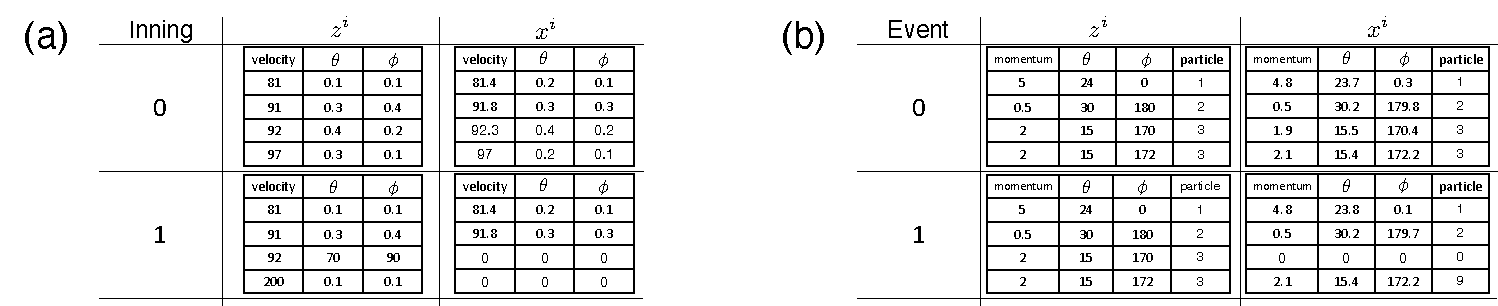
\includegraphics[width=0.8\linewidth]{dataDescription.pdf}
  \caption{The first two rows of (a) toy model data with a pitcher and a catcher, (b) actual data with particles.}
  \label{data}
\end{figure}

In our data, the pitcher's record corresponds to our generated event particle features, and the catcher's record corresponds to the results of MC simulation. The results of each simulation are essentially encoded particle kinematics. One particle has a 4 dimensional vector, where 3 dimensions come from (momentum, polar angle $\theta$, azimuthal angle $\phi$) and another one from particle species. The example of the first two events are in Fig.~\ref{data}-b. In summary, $x^i$'s are in $n\times\{4\times$4\}, and $z^i$'s are also in $n\times\{4\times$4\} dimension, when $n$ is total number of events. Since determining $x^i$ by calculating incremental timesteps is very computationally expensive as mentioned earlier, we aim to replace this step with a generative model that takes input as $z^i$, and outputs $x^i$.

% Relevant related work? (brief summary)
There have been some attempts to generate $x^i$'s using several generative models including the GAN (\citet{Paganini2017}) for different particle experiments. However, the GAN is not an optimal choice for this problem as our goal is to generate a large output dataset and only require relatively low fidelity for each individual output $x^i$, rather than generate only a handful of very high fidelity output events. More recently, the normalizing flow (NF) (\citet{papamakarios2019normalizing}) was studied as a generative model suitable for producing a large number of items that pertain to a very particular distribution of $g: z\rightarrow x$ (\citet{9089305}). \citet{PhysRevD.101.076002} showed that the Nonlinear Independent Component Estimation (NICE) (\citet{Dinh15}) as NF performed well by comparing the technique to existing methods in terms of efficiencies that was defined as average weight during the generation.

% What methods will you try and compare?
We will use a NF model which takes $Z=\{z^i\}$ with the base distribution $p(z)$, and $X=\{x^i\}$ with the target distribution $p(x)$. The mapping in the generative direction is defined as $g:Z\rightarrow X$ with its inverse in normalizing direction $f:X\rightarrow Z$. The distributions have following relation with $f$ and $g$: $p(x)= p(z)|\frac{\partial f}{\partial x}| =  p(z)|\frac{\partial g}{\partial z}|^{-1}$. Technically, it is useful to define $g$ and $f$ as composite bijective functions, $g= g_N \circ g_{N-1}\circ ... \circ g_1$, and $f= f_1 \circ ... \circ f_{N-1} \circ f_N$. With this, it is possible to perform the exact log-likelihood evaluation: $\log p(x) = \log p(z) + \sum\limits_{i=1}^N \log|\frac{\partial f_i}{\partial z_i}|$ where $z_i$ is the $i$-th intermediate flow as $z_i=g_i \circ ... \circ g_1(z) = f_{i+1}\circ ...f_N(x)$. Among possible flow models, we plan to use NICE, and will compare the NF-generated data to the output of the MC simulation.

% What computational resources will you use? Think about time and feasibility.
Regarding the computational feasibility of this project, our group has access to several powerful computing farms, such as LHC Tier-2 \footnote{monitored at http://www.cmsaf.mit.edu/condor4web/}, JLab iFarm \footnote{monitored at https://scicomp.jlab.org/scicomp/index.html\#/farmJobs/activeJob}, and EAPS - MGHPCC \footnote{https://www.mghpcc.org/}. Data storage is not a limiting factor, as 1 GB alone stores 10M $z^i$ - $x^i$ pairs. We propose the following project timeline:\\
\textbf{March 31} Match components of the NICE to our data at pseudo code level, begin implementation \\
\textbf{April 10} - Have basic working example, begin improving and optimizing project \\ 
\textbf{April 25} Conclude developing project flow, begin generating and validating final data \\
\textbf{May 4} - Conclude production run of project, begin finalizing reports.
%OLD:
%We, as members of the MIT Hadronic Physics group, are granted access to MIT clusters such as an HTCondor farm, LHC Tier-2 \footnote{monitored at \url{http://www.cmsaf.mit.edu/condor4web/}}, and a slurm farm, EAPS cluster. Some farms external to MIT can be accessed using OSG for CLAS12 collaboration. The ifarm also offers some computing power \footnote{monitored at \url{https://scicomp.jlab.org/scicomp/index.html\#/farmJobs/activeJob}}. These farms are operating anytime. Especially, the EAPS cluster runs without any delay, and supports disk space of 2 TB quota. For $n$ = 5M, $Z$ and $X$ take roughly 400 MB space.

% What is your project plan? You may include key steps and rough internal deadlines for each step.
%\begin{center}
%\begin{tabular}{ c c c }
%\textbf{Date} & \textbf{Project Milestone} \\ 
%  \textbf{March 31} & Match all components of the NICE to our data in pseudocode level \\
%  \textbf{April 10} & Write an actual code, and have minimal working example on small dataset  \\  
%  \textbf{April 25} & Have working example on full scope of problem \\ 
%  \textbf{May 4} & Conclude production run of project, begin finalizing reports
%\end{tabular}
%\end{center}

% What are the risks? What might turn out to be more difficult than you anticipated? And how might you mitigate these risks?
One anticipated difficulty in this project is that any NF model requires $g$ to be invertible and differentiable. This is fulfilled if we take $x^i$ only when fully reconstructed, like event 0 of Fig.~\ref{data}-b. If not all, but some particles are missing, like event 1 of Fig.~\ref{data}-b, and we encode the momentum feature to 0, differentiability is not guaranteed. Moreover, if all particles are missing, we surely lose invertibility. To address this, we will being work only with fully reconstructed events, which make up the great majority of our interest.  For the events with missing particles, we can encode their momenta to (0, 0, 0) +  small random noises, which can be finally decoded as missing particles, but it is not clear at this stage if this will be a successful approach. If it is not, we will still be able to learn a great deal about our detector by examining the fully reconstructed cases.
%\quad The overarching goal of this project is to provide a correction factor for detector acceptance in our experiment. This will be a large, overall normalization factor, and as our thesis goal is to measure absolute quantities (rather than ratios) this project runs the risk of providing an inaccurate acceptance correction term, which would then yield a significantly shifted final result. This can be mitigated by extensive cross-validation of results, and can be extensively verified by running large simulations in a small region of phase space to create new data for comparison purposes.

%\quad On a more technical level, as this is a very high dimensional problem, it could be difficult to engineer an efficient algorithm for this process. This issue could be mitigated by building up to our actual process in incremental steps, e.g., trying to build an algorithm that will be able to efficiently predict the outcome of just one simulated particle, and then build onto more complex initial and final states. If we are not able to realize our full initial and final state mappings to yield correction factors, we would still be able to gain useful insight by understanding better how single particles, e.g. electrons, traverse through our detector. 



%garbages previously submitted <3
%Since the experimental discovery of the proton by Ernest Rutherford over 100 years ago, there have been various attempts to reveal its internal structure. Yet, its three dimensional profile is still elusive. Measurements on deeply virtual exclusive processes (DVEP) from electron-proton scattering are one proposed way to project the proton structure [\citet{PhysRevD.55.7114}]. In the CLAS12 detector at Thomas Jefferson National Accelerator Facility (JLab), experimental data has been taken of these and other processes [\citet{BURKERT2020163419}].

%Ideally, an event should consist of initial and final states. This is not always true because particles in final states are stochastically detected, depending on their kinematics and detector efficiencies.

 %In this work, we match events $x^i$'s into binary labels $y^i$'s: (\textit{A}) events where every particle gets detected and is correctly classified as the final state of the exclusive process of interest; (\textit{B}) events that fail to be classified as the final state but come from the exclusive process. The goal of this work is to estimate the detector acceptance, the number of \textit{B} events based on measurements of \textit{A} events.  %; and (\textit{C}) events that are not related to the exclusive processes. 
 
 %commented by Sangbaek
 %In the real experiment, the number of events labelled as \textit{A} can be measured. On the other hand, it is hard to estimate the number of events labelled as \textit{B} from the experiment. One widely accepted way is to use a Monte-Carlo simulated data set to estimate the detector acceptance [\citet{PhysRevLett.115.212003, 10.1093/ptep/ptaa104}]. The simulation consists of two steps. The first step is to generate physical events by the Metropolis-Hastings algorithm. The second step is to pass these events to the GEANT4 package [\citet{AGOSTINELLI2003250}], which simulates the interaction between the final states and detectors. The experimental data is stored in the JLab computing facility, which can be accessed by ssh-ing into their farm, named ifarm. Simulated data can also be achieved using computing facilities connected to Open Science Grid (OSG), including MIT farms. The simulated data of a few million events are already achieved, more amounts of simulated data can be easily taken from OSG. For example, in one day, we can roughly simulate 100M events of data.


%Unlike our physics process of interest, which has a high dimensional phase space, most physics final states are considerably more simple, and as such, it has been easier for previous experiments to just run GEANT4 simulations, rather than use machine learning to determine acceptance corrections. As such, work exactly similar to our proposed project has not yet been performed, but machine learning techniques are ubiquitous throughout our research community. Convolutional neural networks (CNN) have been explored by the ALICE collaboration at CERN to supplement particle identification algorithms [\citet{Viljoen2020}], essentially analogous to our project except we will classify whole events, rather than individual particles. Moreover, research is ongoing with replacing traditional GEANT4 simulations with ML boosting to produce 'fast simulations' wherein computationally expensive simulation over dense detector materials are replaced with GANs and VAEs to yield orders of magnitude speedup in simulation time [\citet{Albertsson2018}, \citet{Paganini2017}].


%There are difficulties in estimating the detector acceptance using simulated data. Generally, this type of computing takes too much time to collect significant statistics. Also, sometimes kinematics of label \textit{A} events in simulation may not match with label \textit{A} events in the real experiment. Also, the ratio from simulated data largely depends on theoretical model for probability distribution that was used for Metropolis-Hastings algorithm. Finally, the acceptance only depends on particle kinematics, so it is not efficient to run each process for large statistics. Now this task can be re-defined as a machine learning problem in following way. We have particle momenta in the experimental and simulated data. As indicated earlier, the detector acceptance, despite being stochastic, must be a function of momenta of final states. We take momenta of final states as feature vectors. Each event has label of detector acceptance $\in$ [0, 1], by definition. We define training data sets as simulated data, and a test data set as experimental data. We keep cross validate with several training data sets, and apply our algorithm to the test data.

%Like previous works, we propose using CNN and GAN for this project. First, we will try regression with CNN with simulated data, and test on experimental data. Second, we will try GAN to mimic our simulated data to get more statistics without performing more simulation. We will estimate the detector acceptance with GAN data, and compare the detector acceptance for the experimental data.
